\documentclass[aspectratio=169,11pt]{beamer}

\usepackage[T1]{fontenc}
\usepackage{lmodern}
\usepackage{booktabs}
\usepackage{array}
\usepackage{hyperref}

% ---------------------------------------------------------------- design
\definecolor{kred}{RGB}{178,28,36}
\definecolor{kgrey}{RGB}{90,90,90}
\definecolor{klight}{RGB}{247,240,240}

\usetheme{default}
\usecolortheme{default}
\setbeamercolor{structure}{fg=kred}
\setbeamercolor{frametitle}{fg=kred,bg=white}
\setbeamercolor{title}{fg=kred}
\setbeamercolor{itemize item}{fg=kred}
\setbeamercolor{itemize subitem}{fg=kgrey}
\setbeamercolor{alerted text}{fg=kred}
\setbeamertemplate{navigation symbols}{}
\setbeamertemplate{itemize item}{\raisebox{0.15ex}{\tiny$\blacksquare$}}
\setbeamertemplate{itemize subitem}{\raisebox{0.15ex}{\tiny$\square$}}
\setbeamerfont{frametitle}{series=\bfseries,size=\large}
\setbeamerfont{title}{series=\bfseries}
\setbeamertemplate{footline}{%
  \hfill\textcolor{kgrey}{\tiny\insertframenumber}\hspace{2ex}\vspace{1ex}}

\hypersetup{colorlinks=true,urlcolor=kred}

\newcommand{\redline}{\textcolor{kred}{\rule{\textwidth}{1pt}}}

\title{\textbf{HE-OFT}}
\subtitle{Threat model, paper updates, results}
\author{Halil \.{I}brahim Kanpak}
\date{29 July 2026}

\begin{document}

% ================================================================ 1
\begin{frame}[plain]
  \vfill
  {\Huge\textbf{\textcolor{kred}{HE-OFT}}}\\[0.4em]
  {\large One-shot federated fine-tuning under multiparty CKKS}\\[1.2em]
  \redline\\[0.8em]
  {\normalsize Threat model \quad$\cdot$\quad Paper updates \quad$\cdot$\quad Results}\\[1.6em]
  {\small Halil \.{I}brahim Kanpak \hfill 29 July 2026}
  \vfill
\end{frame}

% ================================================================ 2
\begin{frame}
  \begin{columns}[T]
    \begin{column}{0.52\textwidth}
      \begin{itemize}
        \item \textbf{Clients.} They hold private data. They train locally.
        \item \textbf{Server.} It adds ciphertexts. It holds no key.
        \item \textbf{Serving party.} It answers queries. It holds no key.
      \end{itemize}
      \vspace{1em}
      \redline\\[0.6em]
      \textbf{Each client sends one message.}\\
      The message is the encrypted head displacement.\\
      The adapter stays on the client.
    \end{column}
    \begin{column}{0.46\textwidth}
      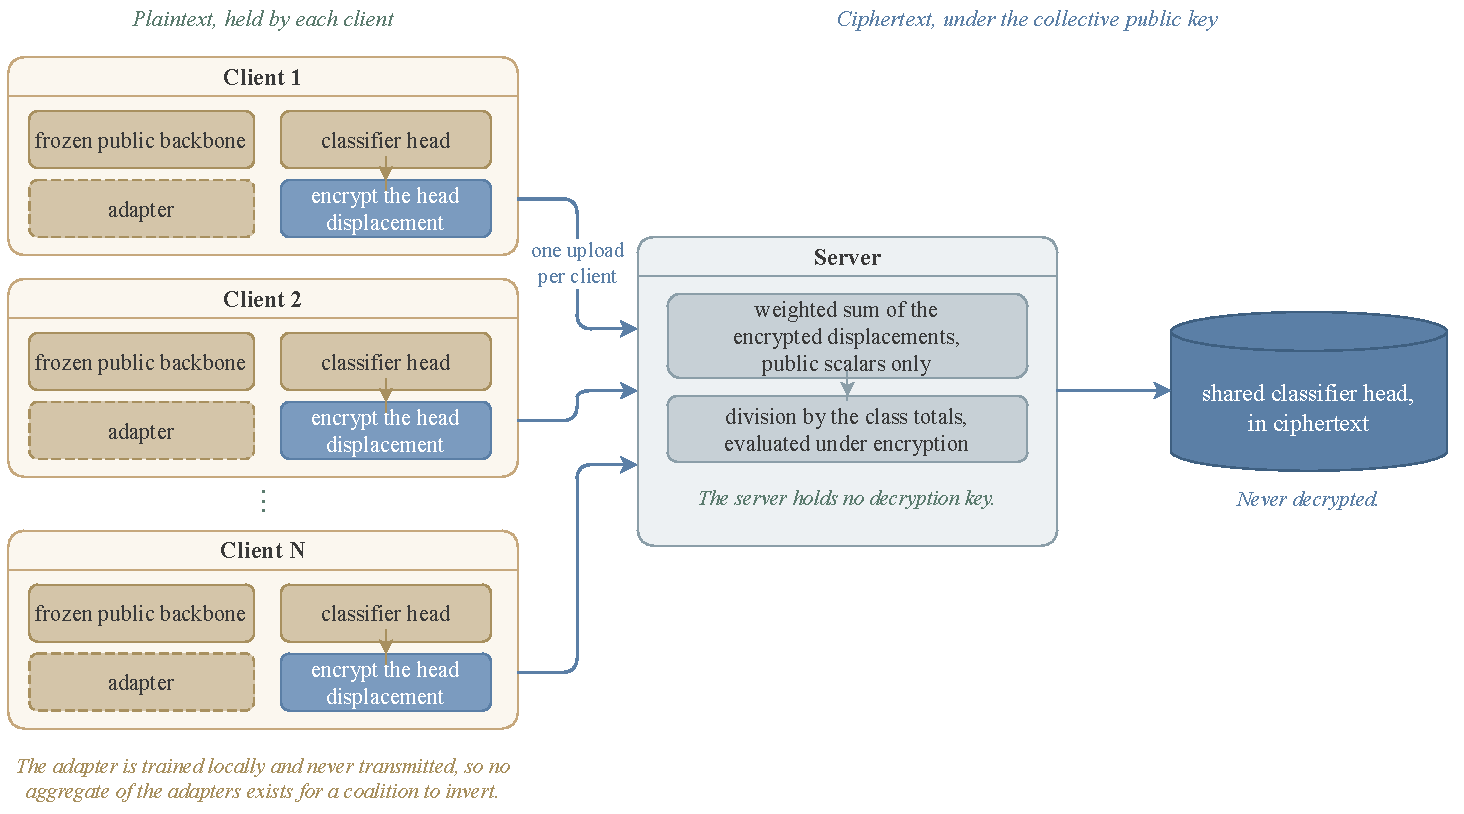
\includegraphics[width=\linewidth]{fig_training.pdf}
    \end{column}
  \end{columns}
\end{frame}

% ================================================================ 3
\begin{frame}
  \begin{itemize}
    \item Every client message is a ciphertext.
    \item The shared head stays a ciphertext. No party decrypts it.
    \item The class totals stay encrypted. The server inverts them under encryption.
    \item Decryption needs a share from every client.
  \end{itemize}
  \vspace{0.8em}
  \redline\\[0.6em]
  \textbf{Collusion.} A group of $N-1$ clients plus the server cannot decrypt.
  \begin{itemize}
    \item No adapter sum exists. The group has nothing to subtract.
    \item The head is never plaintext. The group cannot invert it.
    \item The totals are never plaintext. The group cannot read the last histogram.
  \end{itemize}
\end{frame}

% ================================================================ 4
\begin{frame}
  \begin{columns}[T]
    \begin{column}{0.5\textwidth}
      \begin{itemize}
        \item The client computes its own features.
        \item It sends them encrypted.
        \item The serving party applies the head.
        \item It takes the argmax under encryption.
        \item A quorum sends the label to the asker alone.
      \end{itemize}
      \vspace{0.8em}
      \redline\\[0.6em]
      The client learns the labels it asks for.\\
      \textbf{This is the only channel left.}
    \end{column}
    \begin{column}{0.48\textwidth}
      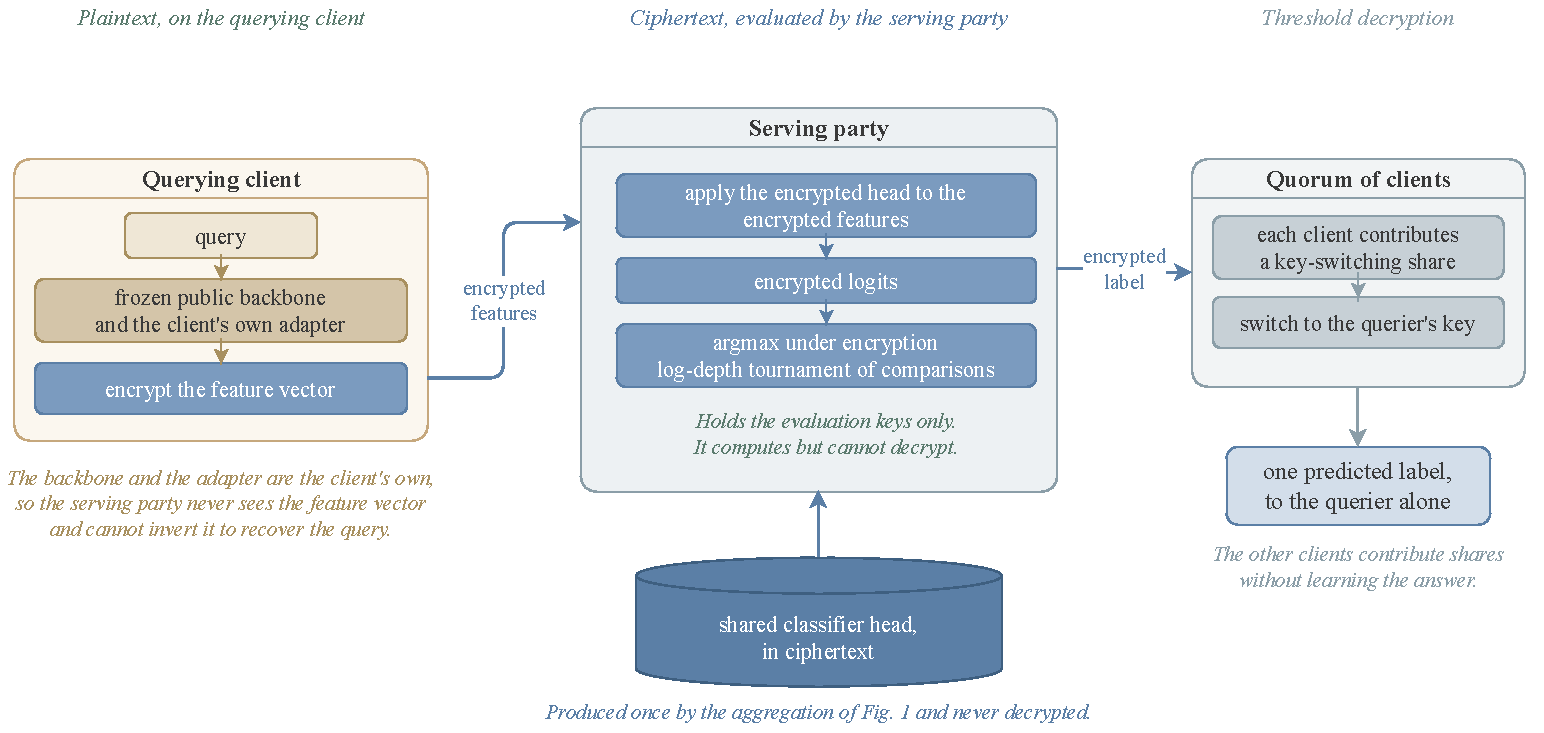
\includegraphics[width=\linewidth]{fig_serving.pdf}
    \end{column}
  \end{columns}
\end{frame}

% ================================================================ 5
\begin{frame}
  \textbf{We return an index. We do not return scores.}
  \vspace{0.8em}
  \begin{itemize}
    \item The head is linear in features the client computes.
    \item Scores give a linear system. $d+1$ queries solve it. Here $d+1=769$.
    \item An index gives about $\log_2 C$ bits. The adversary must search.
  \end{itemize}
  \vspace{1em}
  \redline\\[0.6em]
  \textbf{Carlini et al., ICML 2024.} They stole the final projection layer of a
  production language model for under \$20.
  \begin{itemize}
    \item Their attack needs log-probabilities \emph{and} a logit bias.
    \item OpenAI and Google then restricted that combination.
    \item \alert{We never offer it. This is construction, not policy.}
  \end{itemize}
\end{frame}

% ================================================================ 6
\begin{frame}
  We measured it. The adversary is a client. It queries and fits a linear model.
  \vspace{0.5em}
  \begin{center}
  \footnotesize
  \begin{tabular}{lccccccc}
    \toprule
    Task & $C$ & majority & $10^3$ & $5\!\cdot\!10^3$ & $2\!\cdot\!10^4$ & $5\!\cdot\!10^4$ & $2\!\cdot\!10^5$\\
    \midrule
    AG-News   & 4  & 0.488 & 0.635 & 0.823 & 0.936 & 0.973 & 0.993\\
    DBpedia   & 14 & 0.250 & 0.387 & 0.612 & 0.804 & 0.901 & 0.971\\
    Banking77 & 77 & 0.083 & 0.174 & 0.355 & 0.592 & 0.755 & 0.900\\
    \bottomrule
  \end{tabular}
  \end{center}
  \vspace{0.6em}
  \redline\\[0.6em]
  \begin{itemize}
    \item Fidelity means agreement with the served model, not task accuracy.
    \item Cost tracks the head size $C\,d$. Fidelity 0.90 costs 3 to 5 queries per parameter.
    \item \alert{A deployment sets its query allowance from $C$ and $d$.}
    \item Small label spaces are the tight case. A small head is cheap to copy.
  \end{itemize}
\end{frame}

% ================================================================ 7
\begin{frame}
  \begin{center}
  \footnotesize
  \begin{tabular}{llccc}
    \toprule
    Answer & $\varepsilon$ & Model accuracy & Copy fidelity \\
    \midrule
    index        & none & 0.649 & 0.989 \\
    index        & 2    & 0.494 & 0.889 \\
    index        & 0.5  & 0.303 & 0.598 \\
    \midrule
    distribution & none & 0.649 & \alert{1.000} \\
    distribution & 8    & 0.266 & 0.484 \\
    \bottomrule
  \end{tabular}\\[0.3em]
  \tiny AG-News, mean over three seeds, $10^5$ queries.
  \end{center}
  \vspace{0.4em}
  \redline\\[0.6em]
  \begin{itemize}
    \item The honest user pays the noise on every query.
    \item The adversary averages the noise away over many queries.
    \item Damage grows with the class count. The model breaks before the attack does.
    \item \alert{The query allowance is the control. Noise is not a substitute.}
  \end{itemize}
\end{frame}

% ================================================================ 8
\begin{frame}
  \begin{columns}[T]
    \begin{column}{0.5\textwidth}
      \textbf{Threat model}
      \begin{itemize}\small
        \item The model is never disclosed.
        \item Queries return one label.
        \item Prior work now cited for this channel.
      \end{itemize}
      \vspace{0.6em}
      \textbf{New measurements}
      \begin{itemize}\small
        \item Extraction cost against query count.
        \item Encrypted reciprocal: 4.21 s.
        \item Bootstrapping keys: 15.5 MiB, once.
        \item Threshold decryption against $N$.
        \item Label skew and local steps sweep.
      \end{itemize}
    \end{column}
    \begin{column}{0.5\textwidth}
      \textbf{Presentation}
      \begin{itemize}\small
        \item Peer comparison moved to prose.
        \item We compare the cost of the privacy mechanism.
        \item We do not claim the raw accuracy margin.
      \end{itemize}
      \vspace{0.6em}
      \textbf{Why}
      \begin{itemize}\small
        \item Prior work trains a small network from scratch.
        \item We fine-tune a frozen public backbone.
        \item A table would suggest a level comparison.
      \end{itemize}
    \end{column}
  \end{columns}
\end{frame}

% ================================================================ 9
\begin{frame}
  \begin{center}
  \footnotesize
  \begin{tabular}{lccccc}
    \toprule
     & & \multicolumn{2}{c}{servable} & & \\
    \cmidrule(lr){3-4}
    Task & $C$ & shared head & personal adapter & alone & disclosed\\
    \midrule
    AG-News   & 4   & \textbf{0.649} & 0.479 & 0.475 & 0.739\\
    TREC      & 6   & \textbf{0.607} & 0.429 & 0.400 & 0.711\\
    DBpedia   & 14  & \textbf{0.789} & 0.754 & 0.451 & 0.925\\
    Banking77 & 77  & 0.206 & \textbf{0.686} & 0.249 & 0.760\\
    CIFAR-100 & 100 & 0.748 & \textbf{0.774} & 0.197 & 0.784\\
    \bottomrule
  \end{tabular}
  \end{center}
  \vspace{0.6em}
  \redline\\[0.6em]
  \begin{itemize}
    \item Never disclosing the model costs 0.03 to 0.14.
    \item Two arrangements are servable. Neither wins on every task.
    \item The federation picks one without decrypting either.
    \item The rule is right on 13 of 15 cells. It uses no test set.
  \end{itemize}
\end{frame}

% ================================================================ 10
\begin{frame}
  \begin{columns}[T]
    \begin{column}{0.46\textwidth}
      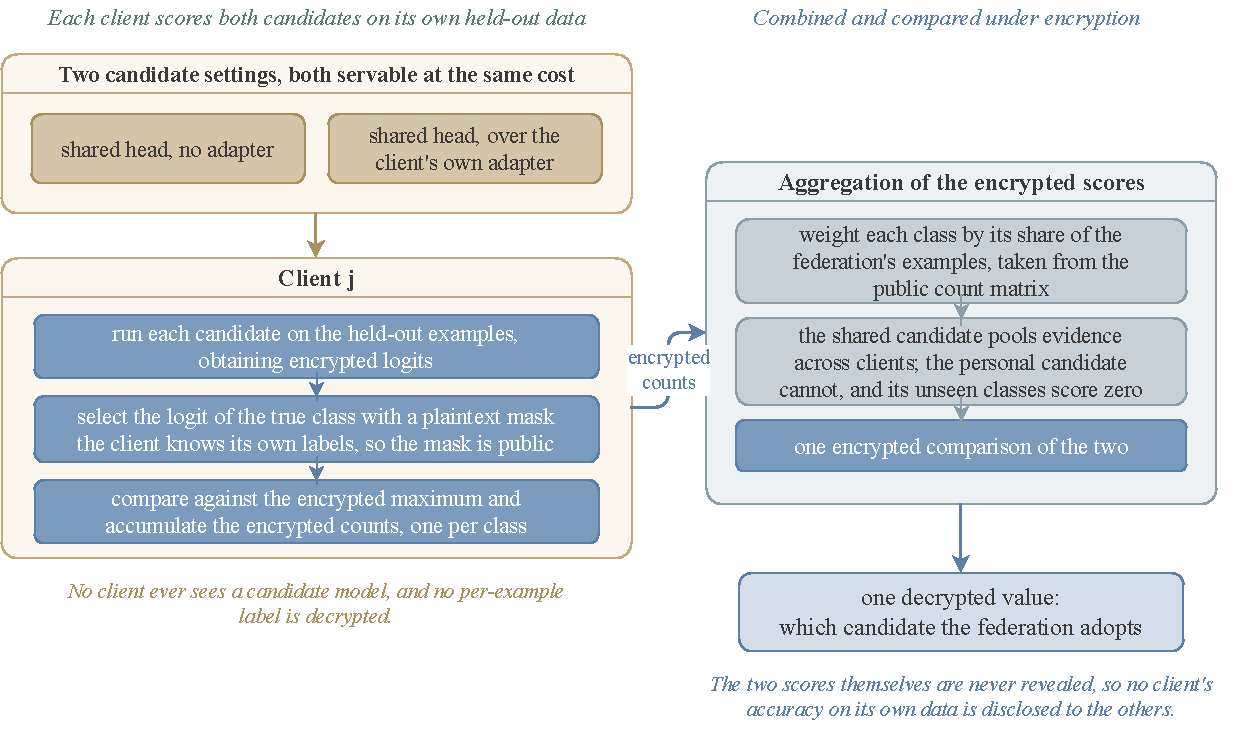
\includegraphics[width=\linewidth]{fig_selection.pdf}
    \end{column}
    \begin{column}{0.52\textwidth}
      \textbf{The direct vote fails.}
      \begin{itemize}\small
        \item Each client scores both on its own data.
        \item That data follows the client's own skew.
        \item The vote picks the personal adapter every time.
        \item It is wrong on 9 of 15 cells.
      \end{itemize}
      \vspace{0.6em}
      \textbf{The estimator works.}
      \begin{itemize}\small
        \item Score both under the federation class prior.
        \item The shared head pools evidence. The personal one cannot.
        \item Unseen classes score zero. This is a lower bound.
        \item One value is decrypted: the winner index.
      \end{itemize}
    \end{column}
  \end{columns}
\end{frame}

% ================================================================ 11
\begin{frame}
  \begin{columns}[T]
    \begin{column}{0.48\textwidth}
      \textbf{Per operation}
      \begin{center}\footnotesize
      \begin{tabular}{lr}
        \toprule
        head on encrypted query & 35.2 ms\\
        head on plaintext query & 4.8 ms\\
        rotation                & 30.8 ms\\
        encrypted reciprocal    & 4.21 s\\
        key switch, $N=10$      & 181 ms\\
        \bottomrule
      \end{tabular}
      \end{center}
      \vspace{0.4em}
      \small We implement the protocol in real multiparty CKKS. We do not simulate it.
    \end{column}
    \begin{column}{0.48\textwidth}
      \textbf{Communication, $N=10$}
      \begin{center}\footnotesize
      \begin{tabular}{lr}
        \toprule
        setup keys, once  & 91 MiB\\
        bootstrap keys, once & 15.5 MiB\\
        per query, total  & \textbf{5.0 MiB}\\
        \bottomrule
      \end{tabular}
      \end{center}
      \vspace{0.4em}
      \begin{itemize}\small
        \item Threshold decryption is linear in $N$: 18 ms and 2.0 MiB per client.
        \item Local refresh replaces 510 MiB per query with 15.5 MiB once.
        \item A GPU gives about $5\times$ on the primitives at matched ring degree.
      \end{itemize}
    \end{column}
  \end{columns}
\end{frame}

% ================================================================ 12
\begin{frame}
  \begin{center}
  \footnotesize
  \begin{tabular}{@{}p{5.3cm}p{3.1cm}p{4.3cm}@{}}
    \toprule
    \textbf{Venue} & \textbf{Next deadline} & \textbf{Link}\\
    \midrule
    NDSS 2027                & 19 Aug 2026 & \href{https://www.ndss-symposium.org/}{ndss-symposium.org}\\
    USENIX Security 2027     & 25 Aug 2026 & \href{https://www.usenix.org/conference/usenixsecurity27}{usenix.org}\\
    IEEE S\&P 2027           & 17 Nov 2026 & \href{https://sp2027.ieee-security.org/}{sp2027.ieee-security.org}\\
    ACM CCS 2027             & not announced & \href{https://www.sigsac.org/ccs/CCS2027/}{sigsac.org}\\
    \addlinespace[0.9em]
    \midrule
    \addlinespace[0.2em]
    AsiaCCS 2027             & 21 Aug 2026 & \href{https://sec-deadlines.github.io/}{sec-deadlines.github.io}\\
    PETS 2027                & 31 Aug 2026 & \href{https://petsymposium.org/cfp27.php}{petsymposium.org}\\
    DSN 2027                 & 2 Dec 2026  & \href{https://sec-deadlines.github.io/}{sec-deadlines.github.io}\\
    EuroS\&P 2027            & see call    & \href{https://www.ieee-security.org/Calendar/cfps/cfp-EuroSnP2027.html}{ieee-security.org}\\
    \addlinespace[0.9em]
    \midrule
    \addlinespace[0.2em]
    IEEE TIFS                & rolling & \href{https://www.comsoc.org/publications/journals/ieee-tifs}{ieee.org}\\
    IEEE TNSE  & rolling & \href{https://www.computer.org/csdl/journal/na}{ieee.org}\\
    \bottomrule
  \end{tabular}
  \end{center}
  \vspace{0.3em}
  {\tiny Dates from \href{https://sec-deadlines.github.io/}{sec-deadlines.github.io}, checked 29 July 2026. Confirm on the venue page.}
\end{frame}

% ================================================================ 13
\begin{frame}[plain]
  \vfill
  \begin{center}
    {\Large\textbf{\textcolor{kred}{Open points}}}\\[1.2em]
    \redline\\[1em]
    \begin{minipage}{0.8\textwidth}
      \begin{itemize}
        \item Client count sweep is still running.
        \item Pooled ceiling gives the reference the tables need.
        \item Matched partitions for the private baseline are queued.
      \end{itemize}
    \end{minipage}
  \end{center}
  \vfill
\end{frame}

\end{document}
